Fully-supervised regularization monotonically shrinks the learned value function. Bootstrapped regularization is recursively applied, so \textbf{the value function may counterintuitively increase with $\eta$.}
\vspace{-.17in}
\begin{center}
    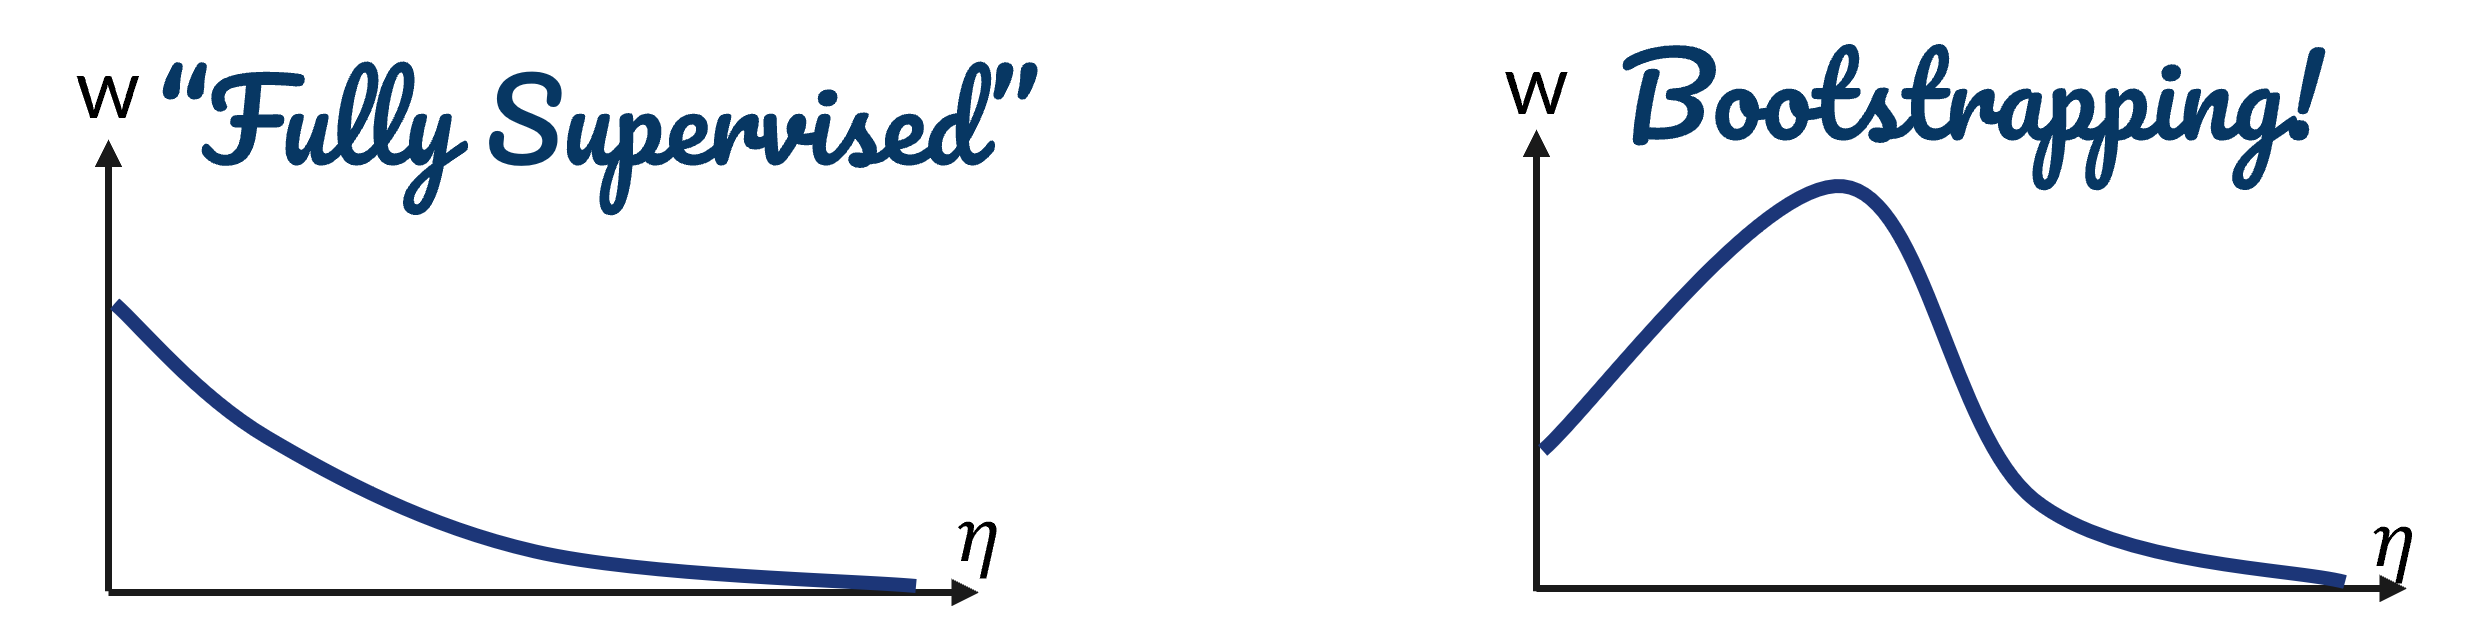
\includegraphics[scale=0.4]{parts/nonmonotonic/illus.png}
\end{center}
\vspace{-.07in}
TD learning may diverge at specific $\eta$, possibly multiple values. For example:
\vspace{-.07in}
\begin{center}
    \hspace*{1in}
    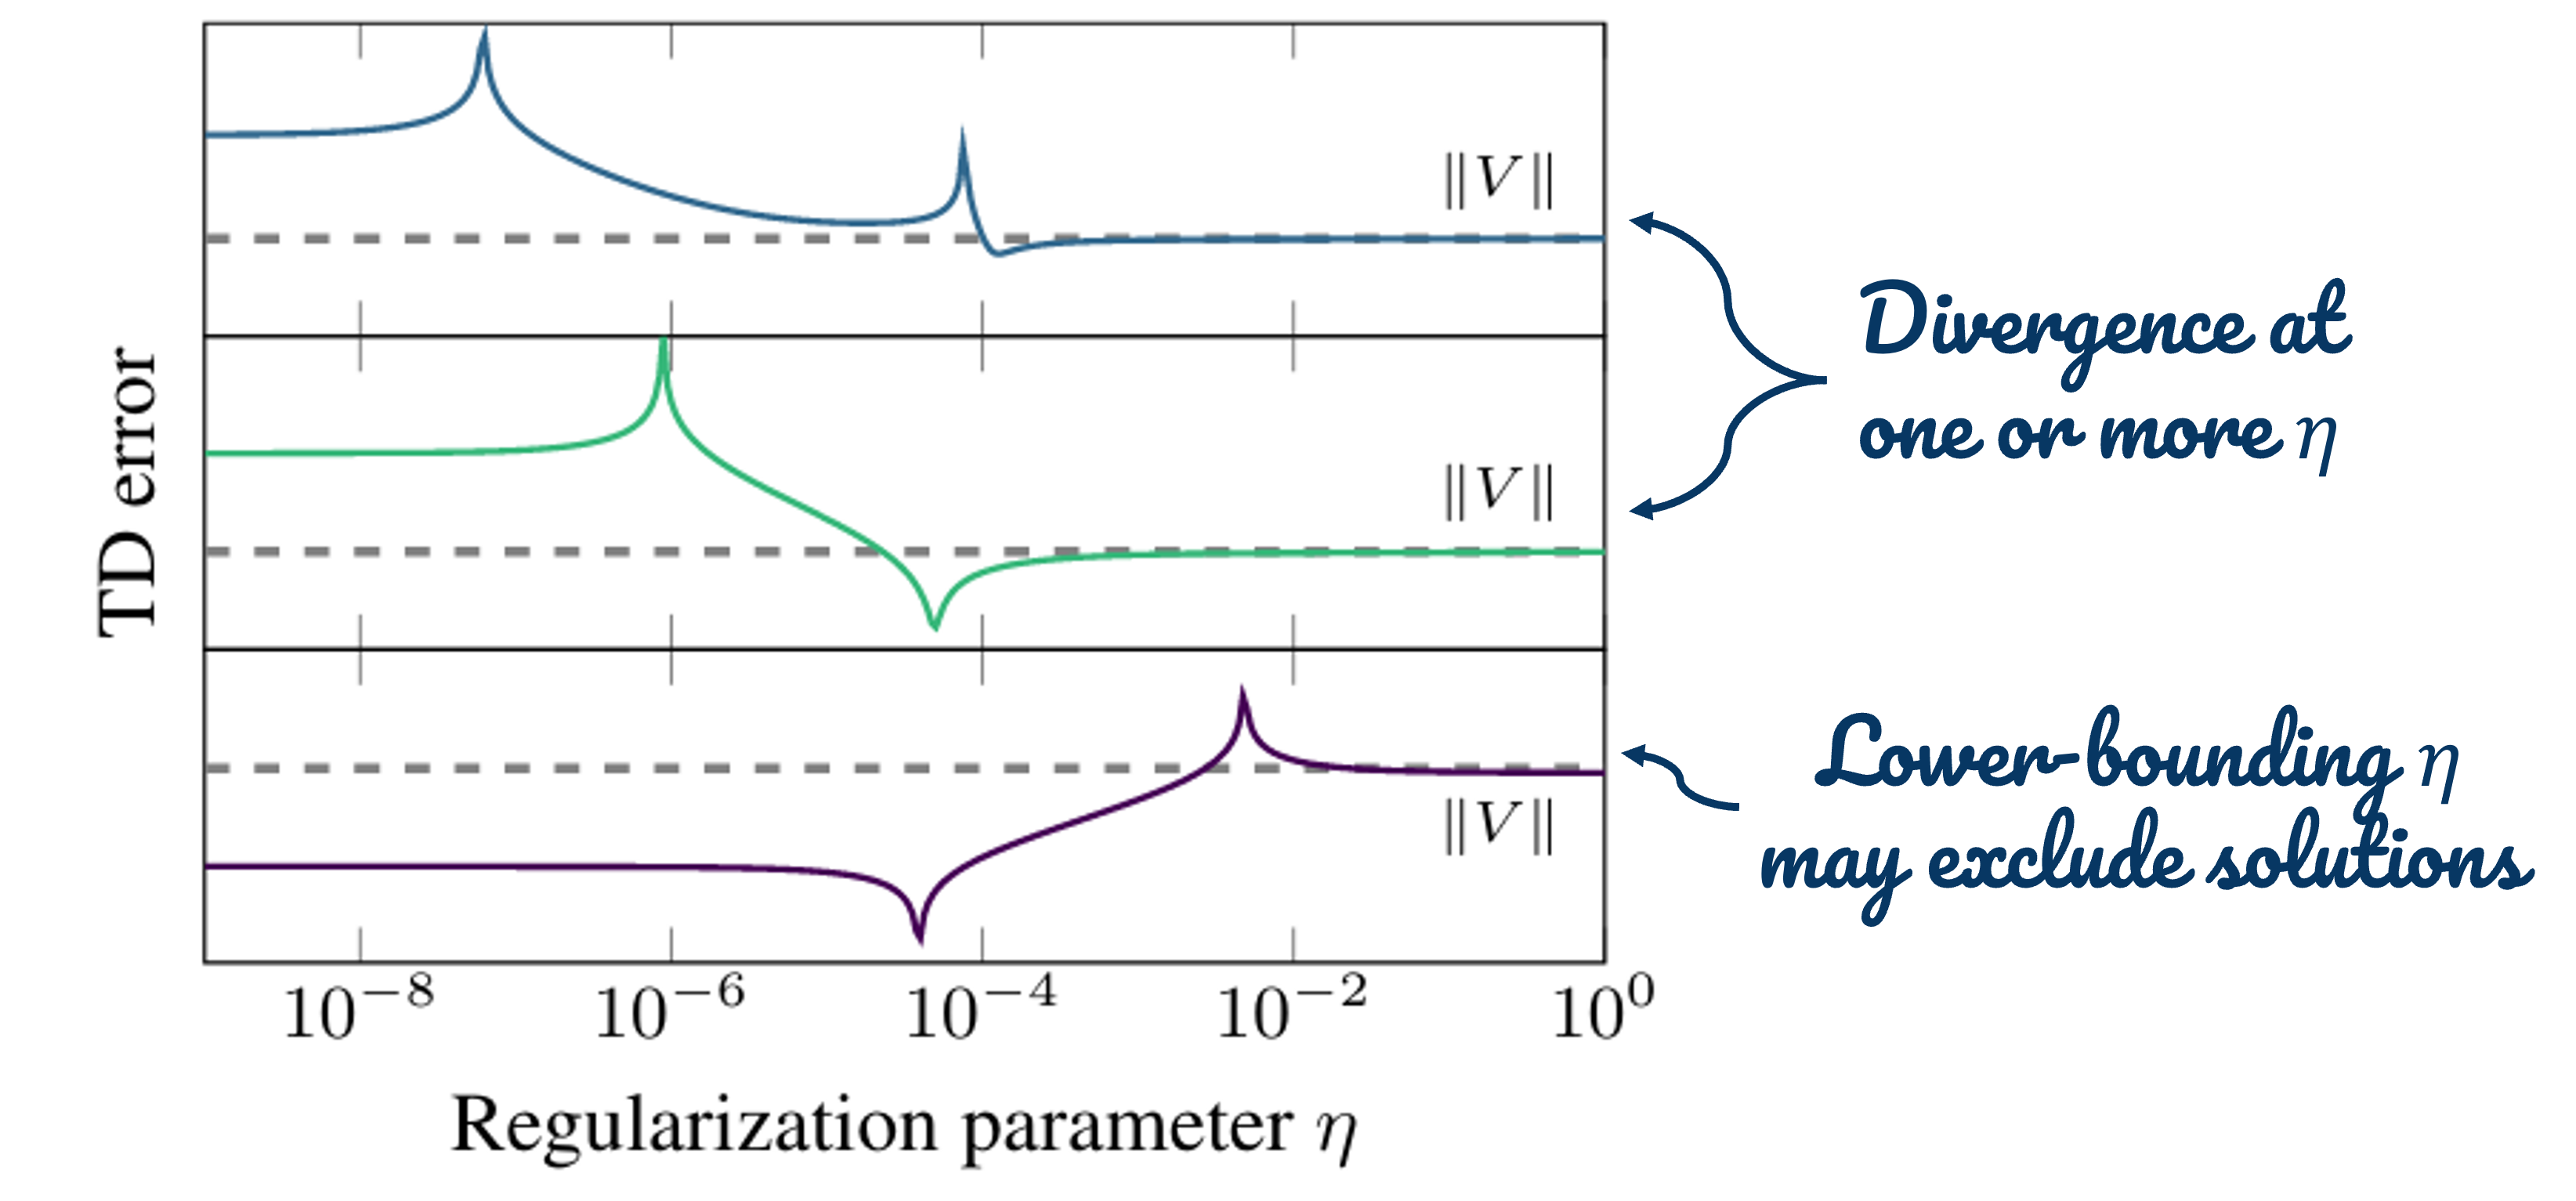
\includegraphics[scale=0.4]{parts/nonmonotonic/threeex.png}
\end{center}
\vspace{-.07in}
A common fix is to assume TD learning behaves ``almost-PSD'' and so lower-bound $\eta$. This assumption is dangerous: it may restrict us to a domain in which TD learning is vacuous.
